\documentclass[12pt]{article}

\usepackage{float}
\usepackage{amsmath}
\usepackage{graphicx}
\usepackage{enumitem}
\usepackage[margin=1.00in]{geometry}
%\usepackage[font=footnotesize]{caption}

\usepackage{bm}
\newcommand{\m}[1]{\mathbf{\bm{#1}}}

\usepackage[longnamesfirst]{natbib} % make it so the first citation
\bibpunct{(}{)}{;}{a}{}{,}

\begin{document}

\noindent Mickey Warner

\noindent AMS 241

\section*{Problem 1}

\subsection*{The DP mixture model}

A simulated dataset consisting of $n=250$ random draws from the mixture of normals $0.2N(-5, 1)+0.5N(0,1)+0.3N(3.5,1)$ will be analyzed in this problem. We consider the location normal Dirichlet process mixture model

\[ f(\cdot|G, \phi) = \int k_N(\cdot|\theta, \phi)dG(\theta),~~~G|\alpha,\mu,\tau^2\sim DP(\alpha, G_0=N(\mu,\tau^2)) \]

\noindent where $k_N(\cdot|\theta,\phi)$ is the density function of a normal distribution with mean $\theta$ and variance $\phi$. Hence, we are mixing over the location of the normal distribution. The hierarchical version of the model is given by 
\begin{align*}
y_i|\theta_i,\phi &\overset{ind}\sim k_N(y_i|\theta_i,\phi),~~~i=1,\ldots,n \\
\theta_i|G &\overset{iid}\sim G,~~~i=1,\ldots,n \\
G|\alpha,\mu,\tau^2 &\sim DP(\alpha, G_0=N(\mu,\tau^2)) \\
\alpha,\mu,\tau^2,\phi &\sim p(\alpha)p(\mu)p(\tau^2)p(\phi) 
\end{align*}

\noindent We let $\alpha\sim Gamma(a_\alpha, b_\alpha)$, $\mu\sim N(a_\mu, b_\mu)$, $\tau^2\sim IG(a_{\tau^2}, b_{\tau^2})$, and $\phi\sim IG(a_\phi, b_\phi)$, where the gamma has mean $a/b$ and the inverse gamma has mean $b/(a-1)$. These lead to easily sampled full conditionals.

Posterior inference is made by sampling from the marginal posterior $p(\m{\theta},\alpha,\mu,\tau^2,\phi|\m{y})$, where $\m{\theta}=(\theta_1,\ldots,\theta_n)$ are the latent mixing parameters and $\m{y}=(y_1,\ldots,y_n)$ are the data. This marginal posterior is found by integrating out the infinite-dimensional parameter $G$ from the full posterior distribution

\[p(\m{\theta},\alpha,\mu,\tau^2,\phi|\m{y}) = \int p(G,\m{\theta},\alpha,\mu,\tau^2,\phi|\m{y})dG \]

\noindent or, rather, by noting that the full posterior may be factored, using Bayes' formula, into a product of the full conditional of $G$ and the marginal posterior

\[ p(G,\m{\theta},\alpha,\mu,\tau^2,\phi|\m{y}) = p(G|\m{\theta},\alpha,\mu,\tau^2,\phi,\m{y})p(\m{\theta},\alpha,\mu,\tau^2,\phi|\m{y}). \]

\subsection*{(part 1) Full conditionals of the marginal posterior}

\noindent To simulate from $p(\m{\theta},\alpha,\mu,\tau^2,\phi|\m{y})$ we iteratively draw from the full conditionals of each parameter $\theta_1,\ldots,\theta_n,\alpha,\mu,\tau^2,\phi$. The expressions for the condtional distributions are based on the P{\'o}lya urn representation. Before we present the distributions, we introduce some notation.

Since $G$ is almost surely discrete there will be a clustering among the $\theta_i$s and the Gibbs sampler we employ takes advantage of this fact. The following list describes the notation used throughout this section:
\begin{itemize}[label=$\cdot$]
\item $n^*$ denotes the number of distinct $\theta_i$s
\item $\theta_j^*$, $j=1,\ldots,n^*$ are the distinct $\theta_i$s
\item $\m{w}=(w_1,\ldots,w_n)$ is the vector that matches each $\theta_i$ to its corresponding $\theta_j^*$, i.e., $w_i=j$ if and only if $\theta_i=\theta_j^*$
\item $n_j$ is the size of the $j$th cluster, $|\{i:w_i=j\}|$, $j=1,\ldots,n^*$
\end{itemize}

\noindent The vectors $(n^*, \m{w}, \theta_1^*,\ldots,\theta_{n^*}^*)$ and $(\theta_1,\ldots,\theta_n)$ are equivalent. The former will simplify the calculations to follow.

For each $\theta_i, i=1,\ldots,n$, the full conditional $p(\theta_i|\{\theta_k:k\neq i\},\alpha,\mu,\tau^2,\phi,\m{y})$ is given by
\[ \frac{\alpha q_0}{\alpha q_0 + \sum_{j=1}^{n^{*-}} n_j^-q_j}h(\theta_i|\mu,\tau^2,\phi,y_i)+\sum_{j=1}^{n^{*-}}\frac{n_j^-q_j}{\alpha q_0 + \sum_{j=1}^{n^{*-}}n_j^-q_j}\delta_{\theta_j^{*-}}(\theta_i) \]
\[ =Ah(\theta_i|\mu,\tau^2,\phi,y_i)+\sum_{j=1}^{n^{*-}}B_j \delta_{\theta_j^{*-}}(\theta_i) \]

\noindent where
\begin{itemize}[label=$\cdot$]
\item $q_j=k_N(y_i|\theta_j^*,\phi)$,
\item $q_0=\int k_N(y_i|\theta,\phi)g_0(\theta|\mu,\tau^2)d\theta$,
\item $h(\theta_i|\mu,\tau^2,\phi,y_i) \propto k_N(y_i|\theta_i,\phi)g_0(\theta_i|\mu,\tau^2)$,
\item $g_0$ is the density of $G_0=N(\cdot|\mu,\tau^2)$, and
\item The superscript ``$^-$'' denotes the appropriate change to $n^{*-}$, $n_j^-$, and $\theta_j^{*-}$ when omitting $\theta_i$ from their calculations.
\end{itemize}

\noindent We update $p(\theta_i|\{\theta_k:k\neq i\},\alpha,\mu,\tau^2,\phi,\m{y})$, for $i=1,\ldots,n$, sequentially by drawing either (1) a new value from $h$ with probability $A$, or (2) $\theta_j^*$ with probability $B_j$ ($A+B_1+\cdots+B_{n^{*-}}=1$). With each update of $\theta_i$ we also update the clustering ``parameters'' $n^*$, $\theta_j^*$, and $n_j$, for $j=1,\ldots,n^*$ ($\m{w}$ is more or less for bookkeeping and isn't explicitly used in the sampling algorithm).

Note that to use the Gibbs sampler we require conjugacy with $k_N$ and $G_0$. Without conjugacy we would have to resort to other methods for updating $\theta_i$, say an algorithm from \cite{neal2000markov}.

The functional form of $q_j$ is simply a normal density
\begin{align*}
q_j = (2\pi\phi)^{-1/2}\exp\left\{-\frac{1}{2\phi}(y_i - \theta_j^*)^2\right\}
\end{align*}

We solve for $q_0$ by integrating out $\theta$ (which has a normal kernel) and re-arranging terms to simplify to a nice normal density
\begin{align*}
q_0 &= \int (2\pi\phi)^{-1/2}\exp\left\{-\frac{1}{2\phi}(y_i-\theta)^2\right\}(2\pi\tau^2)^{-1/2}\exp\left\{-\frac{1}{2\tau^2}(\theta-\mu)^2\right\}d\theta \\
 &= (4\pi^2\phi\tau^2)^{-1/2} \int \exp\left\{-\frac{1}{2\phi}(y_i-\theta)^2-\frac{1}{2\tau^2}(\theta-\mu)^2\right\}d\theta \\
 &= (4\pi^2\phi\tau^2)^{-1/2} \int \exp\left\{-\frac{1}{2\phi\tau^2}\left[\tau^2y_i^2-2y_i\tau^2\theta +\tau^2\theta^2 + \phi\mu^2 - 2\mu\phi\theta + \phi\theta^2\right]\right\}d\theta \\
 &= (4\pi^2\phi\tau^2)^{-1/2} \int \exp\left\{-\frac{1}{2\phi\tau^2}\left[ \theta^2(\phi+\tau^2) -2\theta(\mu\phi+y_i\tau^2)\right] -\frac{\phi\mu^2+\tau^2y_i^2}{2\phi\tau^2}\right\}d\theta \\
 &= (4\pi^2\phi\tau^2)^{-1/2}\exp\left\{-\frac{\phi\mu^2+\tau^2y_i^2}{2\phi\tau^2}\right\} \int \exp\left\{-\frac{\phi+\tau^2}{2\phi\tau^2}\left[ \theta^2 -2\theta\frac{\mu\phi+y_i\tau^2}{\phi+\tau^2}\right]\right\}d\theta \\
 &= (4\pi^2\phi\tau^2)^{-1/2}\exp\left\{-\frac{\phi\mu^2+\tau^2y_i^2}{2\phi\tau^2}\right\} \int \exp\left\{-\frac{1}{2\sigma^*}\left[ \theta^2 -2\theta \mu^* +\mu^{*2} - \mu^{*2}\right]\right\}d\theta \\
& \mathrm{~~~~~~~~~~~~~~~~~~~~~~~~~~~~~~~~~~~~~~~~(where~\mu^*=\frac{\mu\phi+y_i\tau^2}{\phi+\tau^2},~and~\sigma^* = \frac{\phi\tau^2}{\phi + \tau^2})} \\
 &= (4\pi^2\phi\tau^2)^{-1/2}\exp\left\{-\frac{\phi\mu^2+\tau^2y_i^2}{2\phi\tau^2}\right\} (2\pi\sigma^*)^{1/2}\exp\left\{\frac{\mu^{*2}}{2\sigma^*}\right\} \\
 &= (2\pi\phi\tau^2)^{-1/2}\left(\frac{\phi\tau^2}{\phi+\tau^2}\right)^{1/2}\exp\left\{-\frac{\phi\mu^2+\tau^2y_i^2}{2\phi\tau^2} + \frac{(\mu\phi+y_i\tau^2)^2}{2\phi\tau^2(\phi+\tau)}\right\} \\
 &= (2\pi(\phi+\tau^2))^{-1/2}\exp\left\{\frac{-(\phi\mu^2+\tau^2y_i^2)(\phi+\tau^2) + (\mu\phi+y_i\tau^2)^2}{2\phi\tau^2(\phi+\tau^2)}\right\} \\
 &= (2\pi(\phi+\tau^2))^{-1/2}\exp\left\{\frac{-\phi^2\mu^2-\phi\mu^2\tau^2-\phi y_i^2\tau^2-y_i^2\tau^2 + \mu^2\phi^2+2\mu\phi y_i\tau^2 + y_i^2\tau^2}{2\phi\tau^2(\phi+\tau^2)}\right\} \\
 &= (2\pi(\phi+\tau^2))^{-1/2}\exp\left\{\frac{-\phi\mu^2\tau^2-\phi y_i^2\tau^2+2\mu\phi y_i\tau^2}{2\phi\tau^2(\phi+\tau^2)}\right\} \\
 &= (2\pi(\phi+\tau^2))^{-1/2}\exp\left\{-\frac{y_i^2 - 2y_i\mu + \mu^2}{2(\phi+\tau^2)}\right\} \\
 &= N(y_i|\mu, \phi+\tau^2)
\end{align*}

\noindent And thus the bookkeeping was worth it. More importantly, note the conjugacy requirement for the integral to be tractable.

The density function $h(\theta_i|\cdot)$ has essentially already been derived when finding $q_0$. After dropping all the non $\theta_i$ terms, we are left with the part from $q_0$ that was inside the integral. That is, $h$ is a normal distribution with mean $\mu^*$ and variance $\sigma^*$ given above. This completes the marginal posterior for $\theta_i$.

The conditionals for the other parameters are much easier in comparison. We update $\alpha$ by first drawing an auxiliary variable $\eta|\alpha\sim Beta(\alpha+1,n)$ and then drawing from the conditional 
\[\alpha|\eta,n^*,\m{y}\sim\epsilon Gamma(a_\alpha+n^*, b_\alpha-\log\eta) + (1-\epsilon)Gamma(a_\alpha+n^*-1,b_\alpha-\log\eta)\]
\noindent where $\epsilon=(a_\alpha+n^*-1)/(n(b_\alpha-\log\eta)+a_\alpha+n^*-1)$. Draws for $\eta$ are discarded. This update works since $\alpha$ has a gamma prior.

The joint conditional $p(\mu, \tau^2|\m{\theta}^*, n^*, \m{y})\propto p(\mu,\tau^2)\prod_{j=1}^{n^*}g_0(\theta_j^*|\mu, \tau^2)$ is basically the canonical example of Gibbs sampling. Because of our choice of priors and $G_0$, we will update $\mu$ and $\tau^2$ separately. For $\mu|\cdot$, we have
\begin{align*}
p(\mu|\tau^2,\m{\theta}^*, n^*, \m{y}) &\propto \exp\left\{-\frac{1}{2b_\mu}(\mu-a_\mu)^2\right\}\exp\left\{-\frac{1}{2\tau^2}\sum_{j=1}^{n^*}(\theta_j^*-\mu)^2\right\} \\
&\propto \exp\left\{-\frac{1}{2b_\mu}(\mu^2-2a_\mu\mu+a_\mu^2)-\frac{1}{2\tau^2}(\sum_{j=1}^{n^*}\theta_j^{*2}-2\mu\sum_{j=1}^{n^*}\theta_j^*+n^*\mu^2)\right\} \\
&\propto \exp\left\{-\frac{1}{2b_\mu}(\mu^2-2a_\mu\mu)-\frac{1}{2\tau^2}(-2\mu S+n^*\mu^2)\right\},~~~~~(S=\sum_{j=1}^{n^*}\theta_j^*) \\
&\propto \exp\left\{-\frac{1}{2b_\mu\tau^2}(\mu^2\tau^2-2a_\mu\mu\tau^2 - 2\mu Sb_\mu + \mu^2n^*b_\mu)\right\} \\
&\propto \exp\left\{-\frac{1}{2b_\mu\tau^2}(\mu^2(\tau^2+b_\mu n^*) -2\mu(a_\mu\tau^2 + b_\mu S))\right\} \\
&\propto \exp\left\{-\frac{\tau^2+b_\mu n^*}{2b_\mu\tau^2}\left[\mu^2 -2\mu\left(\frac{a_\mu\tau^2 + b_\mu S}{\tau^2+b_\mu n^*}\right)\right]\right\} \\
&\propto \exp\left\{-\frac{1}{2\sigma'}(\mu-\mu')^2\right\},~~~~~(\mu'=\frac{a_\mu\tau^2+b_\mu S}{\tau^2+b_\mu n^*},~\sigma'=\frac{b_\mu\tau^2}{\tau^2+b_\mu n^*})
\end{align*}
Thus $\mu|\cdot \sim N(\mu', \sigma')$. For $\tau^2|\cdot$, we have
\begin{align*}
p(\tau^2|\mu,\m{\theta}^*, n^*, \m{y}) &\propto (\tau^2)^{-a_{\tau^2}-1}\exp\left(-\frac{b_{\tau^2}}{\tau^2}\right)(\tau^2)^{-n^*/2}\exp\left\{-\frac{1}{2\tau^2}\sum_{j=1}^{n^*}(\theta_j^*-\mu)^2\right\} \\
&\propto (\tau^2)^{-(a_{\tau^2}+n^*/2)-1}\exp\left\{-\frac{1}{\tau^2}\left(b_{\tau^2}+\frac{1}{2}\sum_{j=1}^{n^*}(\theta_j^*-\mu)^2\right)\right\}
\end{align*}
which is an $IG(a_{\tau^2}+n^*/2, b_{\tau^2}+\frac{1}{2}\sum_{j=1}^{n^*}(\theta_j^*-\mu)^2)$

Finally, we need the conditional distribution for $\phi$. We have
\begin{align*}
p(\phi|\cdot) &\propto p(\phi)\prod_{i=1}^nk(y_i|\theta_i,\phi) \\
&\propto \phi^{-a_\phi-1}\exp\left(-\frac{b_\phi}{\phi}\right)\prod_{i=1}^n \phi^{-1/2}\exp\left\{-\frac{1}{2\phi}(y_i-\theta_i)^2\right\} \\
&\propto \phi^{-(a_\phi+n/2)-1}\exp\left\{-\frac{1}{\phi}\left(b_\phi+\frac{1}{2}\sum_{i=1}^n(y_i-\theta_i)^2\right)\right\}
\end{align*}
which is an $IG(a_\phi+n/2, b_\phi+\frac{1}{2}\sum_{i=1}^n(y_i-\theta_i)^2)$. This completes the formulation for all necessary full conditionals to sample from the marginal posterior.

An additional, but not necessary, step is included to improve the sampling of the cluster locations $\theta_j^*$. It can be shown that the full conditional for each $\theta_j^*$ is normally distributed with mean and variance
\[ \frac{\phi\mu+\tau^2\sum_{\{i:w_i=j\}}y_i}{\phi+n_j\tau^2},~~~~~\frac{\phi\tau^2}{\phi+n_j\tau^2} \]
Including this step basically rocked my world when I saw how much better the clustering was.

\subsection*{(part 2) Priors for $\phi$, $\mu$, and $\tau^2$}

The priors I decided upon for the analysis are:
\begin{itemize}[label=$\cdot$]
\item $\phi$ -- $a_\phi=3$, $b_\phi=10$ (mean 5, variance 25)
\item $\mu$ -- $a_\mu=0$, $b_\mu=3$ (mean 0, variance 3)
\item $\tau^2$ -- $a_{\tau^2}=3$, $b_{\tau^2}=10$ (mean 5, variance 25)
\end{itemize}
Plots of the posteriors (Fig. 1), along with predictive distributions (Fig. 5), are given at the end of this section (just before problem 2). In choosing these hyperparameters, I wanted something a bit non-informative, but still small since I knew the data didn't contain anything very extreme. The posterior predictive distributions for a new cluster $\theta_0$ and data point $y_0$ seem to appropriately model the data. I did consider other choices of hyperparameters, and these are discussed now.

I do not show the plots for the following analyses. I ran the sampler with some extreme values for the hyperparameters:
\begin{itemize}[label=$\cdot$]
\item $\phi$ -- $a_\phi=3$, $b_\phi=90$ (mean 45, variance 2025)
\item $\mu$ -- $a_\mu=10$, $b_\mu=0.1$ (mean 10, variance 0.1)
\item $\tau^2$ -- $a_{\tau^2}=2.1$, $b_{\tau^2}=0.1$ (mean 0.09, variance 0.08)
\end{itemize}
Interestingly, the posterior for $\tau^2$ was much higher than its prior, having a 95\% hpd of (4.6, 130.7); $\phi$ was bimodal around 5 and 10; and $\mu$ was concentrated close to 10. The number of posterior clusters also dropped dramatically (concentrated around 1 cluster). The posterior predictive showed the new $\theta_0$ be at the three ``main'' locations (-5, 0, 3.5) of the original prior selection, however the predictive $y_0$ was now unimodal around 0 with variance 10.

Again, I ran the sampler with the previous list of hyperparameters, except I changed $b_\mu$ to equal 10. This time, the bimodality in $\phi$ went away, however it was now centered around 10. The posteriors for $\alpha$, $\mu$, $n^*$, and $\tau^2$ went to much more reasonable values (close to what we see in the plots). The posterior predictive distribution for $\theta_0$ was unimodal and $y_0$ was about the same as before. $\phi$ was still too high, which is why I was seeing poor predictions. Since $\phi$ was high (10, when it should really be closer to 1), there was no emphasis on creating clusters away from $\mu$.

I believe my choice of priors (the original list) to be reasonable as they yield appropriate posterior predictive distributions.

\subsection*{(part 3) Prior for $\alpha$}

In choosing several different hyperparameters for $\alpha$, I noticed that the prior had a large impact on the number of distinct clusters $n^*$. For the analysis, I a selected $a_\alpha=b_\alpha=1$, which gives a prior mean of $\alpha$ to be $1$ and variance $1$. This in turn gives an approximate prior mean for $n^*$ to be about $6.1$.

The posterior distribution for $\alpha$ is shown in Fig. 2.

Having a higher prior mean and variance for $\alpha$ did increase the posterior mean and variance. However, the number of clusters $n^*$ and the posterior predictive distributions were not affected by this change. When I put a very tight, low prior for $\alpha$, one with very small mean and variance, the posterior mean for $n^*$ was much smaller, but the posterior predictive distributions remained about the same. This leads me to believe that though $\alpha$ plays a key role in the posterior of $n^*$, it does not have so much of an impact on the other parameters in the model nor on the predictions.

\subsection*{(part 4) Posteriors for $n^*$ and $\theta_i$}

Fig. 2 shows the posterior for $n^*$ (top left) and a heatmap of how the cluster labels $\theta_i$ were grouped (top right). In Fig. 3, I show the mean and equal-tailed 95\% credible interval for each $\theta_i$. Together, these figures show that there are three main clusters that the $\theta_i$'s fall in.

The three main groups might seem contradictory to what we're seeing in the posterior for $n^*$. What is happening is that when new clusters are formed, they are still around the main groups.

In Fig. 5 (left) we see the posterior predictive distribution of a new cluster label $\theta_0$. A simple look at a kernel density estimate of the data would suggest that the distributional shape of $\theta_0$ is appropriate.

\subsection*{(part 5) Posterior predictive for a new $\theta_0$ and new $y_0$}

In Fig. 4 I show the prior predictive distributions for a new cluster $\theta_0$ and a new observation $y_0$. My prior specification results in fairly widespread normal predictive distributions. On the right, I overlay a KDE of the data. This shows that my priors clearly do not capture the shape of the data.

In Fig. 5 we see the posterior predictive distributions for a new cluster and a new observation. Now, we are able to nicely capture the cluster locations as well as the shape of the data. In these plots and in previous ones with a shaded density, the darker blue region denotes the 95\% highest posterior density set. In the predictive distribution of $\theta_0$ we have a set made up of three intervals.
 
\newpage

%\subsection*{Plots for problem 1}

\begin{figure}[H]
\begin{center}
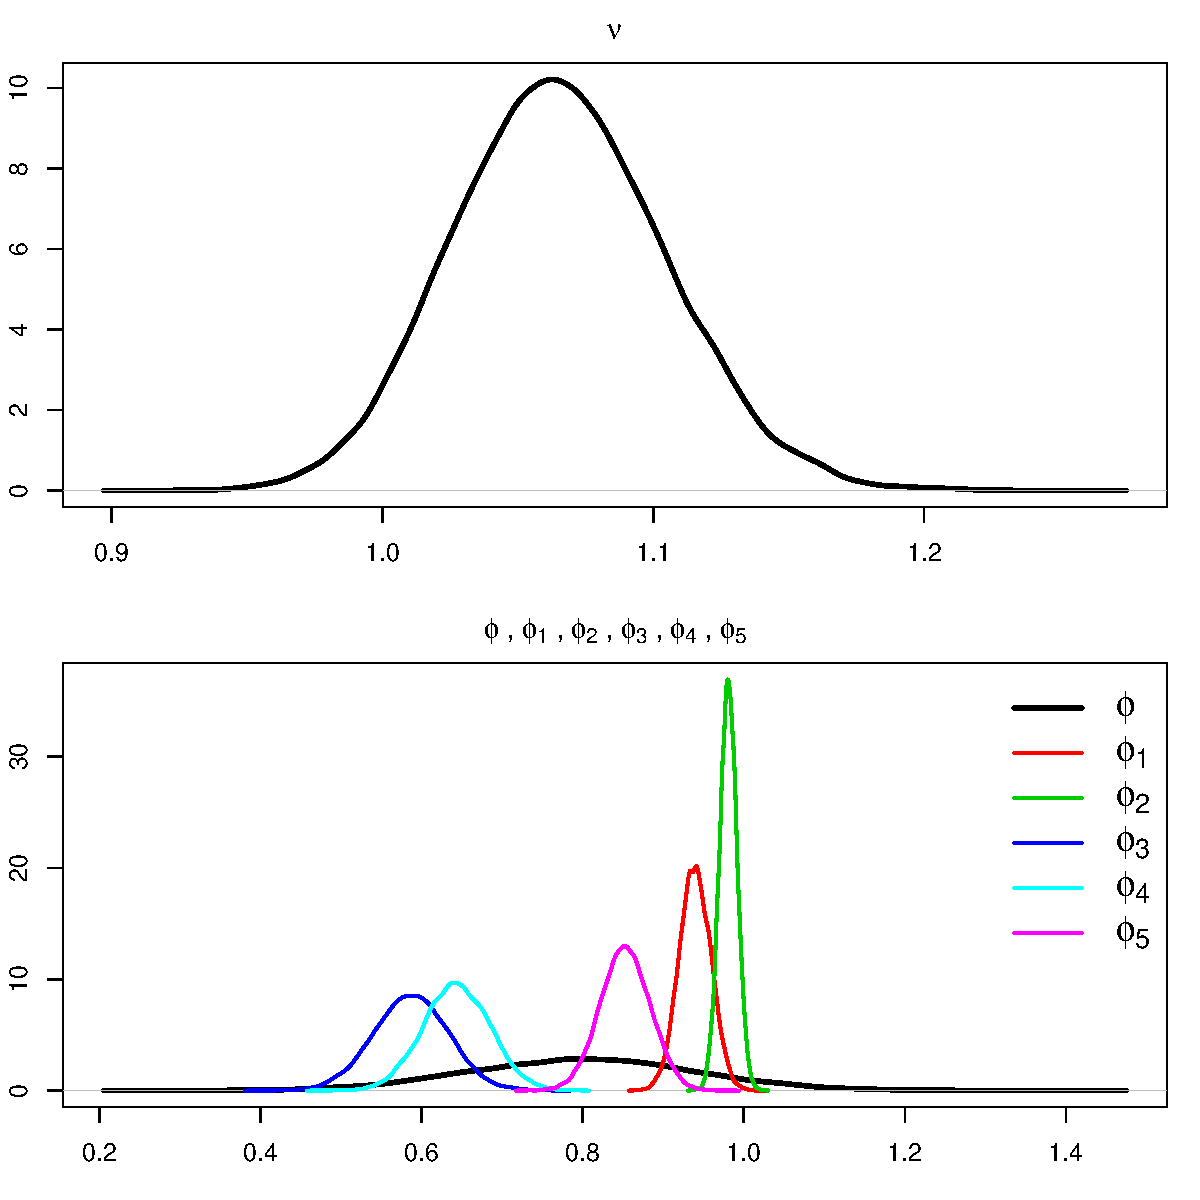
\includegraphics[scale=0.42]{figs/posts_1.pdf}
\caption{Trace plots and posterior distributions for $\phi$, $\mu$, and $\tau^2$}
\end{center}
\end{figure}

\begin{figure}[H]
\begin{center}
\includegraphics[scale=0.45]{figs/nstar_1.pdf}
\caption{Top left: posterior distribution for the number of distinct labels, or clusters, $n^*$. Top right: a heatmap showing how often two labels (or observations) were part of the same cluster; blue denotes fewer times in common and red is for very often paired together. Bottom: (left) trace plot and (right) posterior distribution (and 95\% hpd) for $\alpha$.}
\end{center}
\end{figure}

\begin{figure}[H]
\begin{center}
\includegraphics[scale=0.75]{figs/lines_1.pdf}
\caption{This figure shows each cluster label $\theta_i$, sorted by the order of the observations. Black: equal-tailed 95\% credible intervals for each $\theta_i$. Green: posterior mean for each $\theta_i$. Red: the observations.}
\end{center}
\end{figure}

\begin{figure}[H]
\begin{center}
\includegraphics[scale=0.55]{figs/prior_1.pdf}
\caption{\emph{Prior} predictive distributions for a new cluster $\theta_0$ and new data point $y_0$}
\end{center}
\end{figure}

\begin{figure}[H]
\begin{center}
\includegraphics[scale=0.55]{figs/pred_1.pdf}
\caption{\emph{Posterior} predictive distributions for a new cluster $\theta_0$ and new data point $y_0$. Note the appearance of three ``main'' clusters. Though the posterior for the \emph{number} of clusters $n^*$ showed more than three clusters, most of these were still around the three modes.}
\end{center}
\end{figure}


\newpage

\section*{Problem 2}






\bibliography{refs}
\bibliographystyle{asa}


\end{document}
